% Manuscript source. Numbers are macros from generated/values.tex (scripts/make_paper.py).
% Build:  make paper   (or: python scripts/make_paper.py)
\documentclass[10pt]{article}
\usepackage[a4paper, margin=22mm, top=24mm, bottom=26mm]{geometry}
\usepackage{fontspec}
\usepackage{amsmath, amssymb}
\usepackage{graphicx}
\usepackage{booktabs, tabularx}
\usepackage{xcolor}
\usepackage[font=small, labelfont=bf, labelsep=period, justification=justified,
            singlelinecheck=false]{caption}
\usepackage{titlesec}
\usepackage{enumitem}
\usepackage{microtype}
\usepackage[hidelinks]{hyperref}
\usepackage{fancyhdr}
\usepackage{float}

% ---------------------------------------------------------------- identity
\definecolor{ink}{HTML}{161B1F}
\definecolor{cobalt}{HTML}{2457D6}
\definecolor{vermilion}{HTML}{E33D3F}
\definecolor{muted}{HTML}{8EA8EC}
\definecolor{rule}{HTML}{D9DDE0}
\definecolor{subtle}{HTML}{5B6670}
\color{ink}
\hypersetup{colorlinks=true, linkcolor=cobalt, citecolor=cobalt, urlcolor=cobalt}

\setmainfont{IBMPlexSans}[Path=../.cache/fonts/, Extension=.ttf, UprightFont=*-Regular,
  BoldFont=*-SemiBold, ItalicFont=*-Italic, BoldItalicFont=*-SemiBold]
\setsansfont{IBMPlexSans}[Path=../.cache/fonts/, Extension=.ttf, UprightFont=*-Regular,
  BoldFont=*-SemiBold, ItalicFont=*-Italic, BoldItalicFont=*-SemiBold]
\setmonofont{IBMPlexMono}[Path=../.cache/fonts/, Extension=.ttf, UprightFont=*-Regular,
  BoldFont=*-Medium, Scale=0.9]
\newfontfamily\editorial{Fraunces}[Path=../assets/fonts/, Extension=.ttf,
  UprightFont=*-SemiBold, BoldFont=*-SemiBold]
\newfontfamily\editoriallight{Fraunces}[Path=../assets/fonts/, Extension=.ttf,
  UprightFont=*-Regular]

\usepackage[italic]{mathastext}
\linespread{1.12}
\setlength{\emergencystretch}{2em}
\setlength{\parindent}{0pt}
\setlength{\parskip}{0.55em}
\titleformat{\section}{\editorial\Large\color{ink}}{\thesection}{0.7em}{}
\titleformat{\subsection}{\editorial\large\color{ink}}{\thesubsection}{0.7em}{}
\titleformat{\paragraph}[runin]{\bfseries}{}{}{}[.]
\titlespacing*{\section}{0pt}{1.6em}{0.5em}
\titlespacing*{\subsection}{0pt}{1.2em}{0.35em}
\setlist{itemsep=0.15em, topsep=0.2em}
\captionsetup{labelfont={bf,color=ink}, font={small,color=ink}}
\renewcommand{\arraystretch}{1.15}
\newcommand{\tech}[1]{\texttt{#1}}
\newcommand{\figref}[1]{Fig.~\ref{#1}}

\pagestyle{fancy}
\fancyhf{}
\renewcommand{\headrulewidth}{0pt}
\fancyfoot[L]{\footnotesize\color{subtle}\texttt{Ts65Dn cortical protein signatures}}
\fancyfoot[R]{\footnotesize\color{subtle}\thepage}

% Generated by scripts/make_paper.py from results/ -- do not edit by hand.
\newcommand{\APPfc}{0.23}
\newcommand{\AxisShare}{42}
\newcommand{\AxisShareCI}{0.00--0.48}
\newcommand{\BlockMedian}{0.82}
\newcommand{\BlockPct}{82}
\newcommand{\BlockRange}{0.71--0.88}
\newcommand{\CosCtrlMem}{0.95}
\newcommand{\CosCtrlMemCI}{0.60--0.97}
\newcommand{\CosTsMem}{0.86}
\newcommand{\CosTsMemCI}{0.51--0.94}
\newcommand{\CosTsSal}{0.86}
\newcommand{\CosTsSalCI}{0.42--0.92}
\newcommand{\CtrlShift}{-0.25}
\newcommand{\CtrlShiftCI}{-2.90 to 0.34}
\newcommand{\DSCRfc}{-0.03}
\newcommand{\DYRKfc}{0.18}
\newcommand{\DosageBg}{0.01}
\newcommand{\DosageBgCI}{-0.03 to 0.06}
\newcommand{\DosageDis}{-0.02}
\newcommand{\DosageDisCI}{-0.10 to 0.06}
\newcommand{\DosageExpected}{0.58}
\newcommand{\DosageFold}{1.10}
\newcommand{\DosageFrac}{23}
\newcommand{\DosageQSig}{1}
\newcommand{\DosageRep}{0.66}
\newcommand{\DosageRepTri}{0.70}
\newcommand{\DosageTopFifth}{4}
\newcommand{\DosageTri}{0.13}
\newcommand{\DosageTriCI}{0.06--0.20}
\newcommand{\GroupedBA}{0.602}
\newcommand{\GroupedRFBA}{0.596}
\newcommand{\ICCMedian}{0.72}
\newcommand{\ICCRange}{0.57--0.78}
\newcommand{\ITSNfc}{0.21}
\newcommand{\LearnAtt}{3.1}
\newcommand{\LearnAttP}{0.049}
\newcommand{\LearnRelCtrlMem}{0.84}
\newcommand{\LearnRelCtrlMemCI}{0.61--1.18}
\newcommand{\LearnRelTsMem}{1.04}
\newcommand{\LearnRelTsMemCI}{0.67--1.49}
\newcommand{\LearnRelTsSal}{0.67}
\newcommand{\LearnRelTsSalCI}{0.41--1.01}
\newcommand{\LearnResP}{0.008}
\newcommand{\LearnRespCtrlSal}{9.5}
\newcommand{\LearnSD}{1.63}
\newcommand{\LearnTopProteins}{SOD1, pERK, ARC, IL1B, CaNA, SNCA}
\newcommand{\MagDrugCtrl}{1.5}
\newcommand{\MagDrugTs}{3.0}
\newcommand{\MagTri}{3.8}
\newcommand{\MissingInformative}{0}
\newcommand{\MissingTested}{49}
\newcommand{\MouseMeanBA}{0.613}
\newcommand{\NAffected}{3}
\newcommand{\NAttEighty}{10}
\newcommand{\NBackground}{62}
\newcommand{\NBoot}{4{,}000}
\newcommand{\NCond}{46}
\newcommand{\NGeno}{4}
\newcommand{\NGxC}{9}
\newcommand{\NGxCxT}{3}
\newcommand{\NGxT}{0}
\newcommand{\NImputed}{2}
\newcommand{\NLearnCS}{17}
\newcommand{\NLearnTM}{27}
\newcommand{\NLearnTS}{6}
\newcommand{\NMice}{72}
\newcommand{\NNetPerm}{2{,}000}
\newcommand{\NPanel}{70}
\newcommand{\NPerm}{5{,}000}
\newcommand{\NPersist}{1}
\newcommand{\NProteins}{77}
\newcommand{\NRows}{1{,}080}
\newcommand{\NThreeOne}{64}
\newcommand{\NThreeTwo}{16}
\newcommand{\NTreat}{2}
\newcommand{\NTriSaline}{3}
\newcommand{\NUnique}{76}
\newcommand{\NetNull}{0.263}
\newcommand{\NetP}{0.15}
\newcommand{\NetPairs}{2{,}415}
\newcommand{\NetPairsSig}{0}
\newcommand{\NetStat}{0.289}
\newcommand{\Persist}{61}
\newcommand{\PersistCI}{-0.01 to 2.73}
\newcommand{\PowAttNine}{79}
\newcommand{\PowThreeOneNine}{18}
\newcommand{\PyVersion}{3.11.9}
\newcommand{\Reliability}{0.59}
\newcommand{\RescueCS}{0.22}
\newcommand{\RescueCSCI}{-3.92 to 3.82}
\newcommand{\RescueFrac}{64}
\newcommand{\RescueFracCI}{-0.01 to 1.71}
\newcommand{\RescueP}{0.019}
\newcommand{\RescueSC}{0.84}
\newcommand{\RescueSCCI}{0.09--2.10}
\newcommand{\RowBA}{0.994}
\newcommand{\SODfc}{-0.15}
\newcommand{\Seed}{2026}
\newcommand{\SklearnVersion}{1.9.1}
\newcommand{\SlopeCorr}{0.74}
\newcommand{\SlopeNaive}{0.43}
\newcommand{\TIAMfc}{0.07}
\newcommand{\DocAuthor}{Noushin}

\hypersetup{pdftitle={Trisomy, learning and memantine leave separable, multivariate signatures
  in the Ts65Dn cortex}, pdfauthor={\DocAuthor}}

\begin{document}

% ---------------------------------------------------------------- title
\begin{flushleft}
{\color{subtle}\small\texttt{RESEARCH ARTICLE}}\par\vspace{0.6em}
{\editorial\fontsize{21}{25}\selectfont Trisomy, learning and memantine leave separable,
multivariate signatures in the Ts65Dn cortex\par}
\vspace{0.7em}
{\editoriallight\large A mouse-level analysis of cortical proteins in the Ts65Dn model of Down syndrome\par}
\vspace{0.9em}
{\small\color{subtle}Reproducible analysis: code, tests and every number in this article are
regenerated by \texttt{make reproduce} from the original UCI workbook.\par}
\end{flushleft}
\vspace{0.4em}
{\color{rule}\rule{\linewidth}{0.6pt}}

\begin{abstract}
\noindent\textbf{Problem.} The UCI Mice Protein Expression dataset records 77 cortical proteins
in a mouse model of Down syndrome (Ts65Dn), in mice that did or did not form a fear memory and
did or did not receive the drug memantine. It is widely used to benchmark classifiers, which
creates two problems. Its \NRows{} rows come from only \NMice{} mice, so random row splits leak
each mouse into both training and test data. And classification accuracy does not answer the
biological questions the experiment was designed to address.
\textbf{Approach.} We treated the mouse as the experimental unit and asked four questions: does
an extra gene copy produce proportionally more protein (Q1)? Does trisomy change the brain's
molecular response to learning (Q2)? Does memantine reverse the effects of trisomy (Q3)? Does
trisomy change how proteins co-vary (Q4)? We combined proteins into one score per mouse,
prevented any mouse from being scored on a direction it helped define, and used mouse-level
bootstrap and permutation tests.
\textbf{Findings.} Holding out whole mice lowered eight-group balanced accuracy from \RowBA{} to
\GroupedBA. (Q1) Across six selected proteins, the mean log$_2$ difference was
\DosageFrac\% of the simple 1.5-fold expectation on the log$_2$ scale.
(Q2) Saline-treated Ts65Dn
mice showed \LearnRelTsSal{} times the control protein response to learning (95\% CI
\LearnRelTsSalCI; $p = \LearnAttP$), while the treated estimate was \LearnRelTsMem{}
($p = \LearnResP$ for the specified contrast). (Q3) The estimated shift toward controls was
\RescueFrac\% of the signature gap, with wide uncertainty (\RescueFracCI).
(Q4) This analysis detected no covariance difference ($p = \NetP$).
\textbf{Conclusion.} The data suggest attenuated measured dosage and a weaker
conditioning-associated signature in untreated trisomic mice. Complete restoration,
drug specificity and covariance equivalence are not established.
\end{abstract}

\begin{figure}[h]
\centering
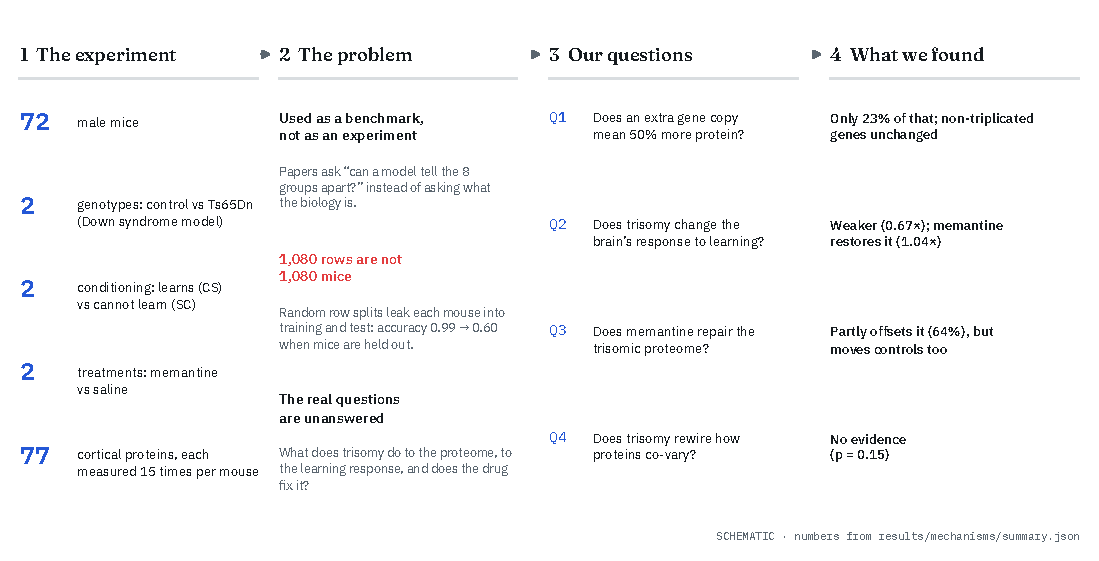
\includegraphics[width=\linewidth]{../results/mechanisms/figures/fig0_overview.pdf}
\caption{\textbf{Study at a glance.} The experiment, the problem with its common use, the four
questions we ask and the short answers. Schematic; numbers are generated from the results.}
\label{fig:overview}
\end{figure}

% ================================================================ 1
\section{Introduction}

\paragraph{Background} Down syndrome, caused by an extra copy of human chromosome 21 (HSA21), is
the most common genetic cause of intellectual disability. The Ts65Dn mouse carries an extra copy
of a segment of mouse chromosome 16 that contains about 90 HSA21 orthologs
\cite{reeves1995, duchon2011, reinholdt2011}. Ts65Dn mice fail context fear conditioning, a test
of associative learning, and acute injection of memantine, an NMDA-receptor antagonist, rescues
that failure \cite{costa2008}. To find the molecular basis of the deficit and its rescue, Ahmed
et al.\ measured 77 proteins and protein modifications in the cortex of Ts65Dn and control mice
after context-shock training (CS: the mouse explores, then is shocked, and learns the
association) or shock-context training (SC: shocked immediately, so no association forms), with
memantine or saline \cite{ahmed2015}. The data were released through UCI \cite{uci2015}.

\paragraph{The problem} The dataset has since been used mainly to benchmark classifiers that
predict a mouse's experimental group. This use has two weaknesses. First, each mouse was measured
15 times, so the \NRows{} rows are not independent samples. Splitting rows at random places
measurements from the same mouse in both training and test data, and the classifier can succeed
by recognising individual mice \cite{lazic2010, kaufman2012}. Second, even a valid accuracy
answers only ``can the groups be told apart?''. It does not say what trisomy does to the
proteome, how the brain responds to learning, or whether the drug repairs anything. These were
the questions the experiment was designed to answer, and they remain open.

\paragraph{Our questions} We analyse the study as a designed experiment, with the mouse as the
unit, and ask:
\begin{enumerate}[label=\textbf{Q\arabic*.}, leftmargin=2.6em]
\item \textbf{Gene dosage.} Do triplicated genes produce 1.5 times as much protein?
\item \textbf{Learning.} Does trisomy change the brain's molecular response to learning, and
  does memantine alter that change?
\item \textbf{Rescue.} Does memantine move the trisomic proteome back toward normal, and is the
  effect specific to trisomic mice?
\item \textbf{Networks.} Does trisomy change how proteins co-vary across mice?
\end{enumerate}
Before answering them we audit the data (Section~\ref{sec:audit}), because the answers depend on
counting mice rather than rows. Fig.~\ref{fig:overview} summarises the study, and
Box~1 defines the main methodological terms.

\begin{figure}[!htb]
\noindent\fcolorbox{rule}{white}{\begin{minipage}{0.97\linewidth}
\small\vspace{0.3em}
{\editorial\normalsize Box 1 \textbullet{} Key concepts}
\begin{description}[leftmargin=0pt, itemsep=0.25em, font=\bfseries]
\item[Experimental unit.] The smallest thing that was independently assigned to a condition:
  here a mouse. Repeated measurements of one mouse are not independent evidence.
\item[Data leakage.] Information from the test data reaching the model during training, which
  makes accuracy look better than it is.
\item[Contrast.] A comparison of group means written as a weighted sum, for example
  Ts65Dn minus control. Every effect in this paper is one.
\item[Signature (axis).] A weighted combination of proteins that captures one effect, such as
  the CS$-$SC difference. Each mouse receives one score along it.
\item[Leave-one-out scoring.] Scoring each mouse on a signature rebuilt without that mouse, so
  a mouse cannot make itself look typical.
\item[Bootstrap / permutation test.] Re-drawing mice to measure uncertainty, and shuffling group
  labels to measure how often chance alone gives an effect as large as the one observed.
\item[False discovery rate ($q$).] The expected share of false positives among the results
  reported as significant when many proteins are tested.
\end{description}
\end{minipage}}
\end{figure}

% ================================================================ 2
\section{Results}

\subsection{Data audit: the mouse is the unit, and replicates are technical}\label{sec:audit}
\textit{Question: what are the independent units, and is the measurement trustworthy?
Answer: 72 mice, each measured 15 times in five technical blocks; the data are usable once
summarised per mouse.}

The workbook contains \NRows{} rows from \NMice{} mice in a balanced $2\times2\times2$ design with
7--10 mice per cell (\figref{fig:design}a). Within each mouse the 15 measurements fall into five
consecutive blocks of three nearly identical rows (\figref{fig:design}b), consistent with three
technical replicates at each point of a five-step dilution series, as used in reverse-phase
protein arrays \cite{tibes2006}. Block membership explains a median \BlockPct\% of
within-mouse variance (IQR \BlockRange), whereas mouse-to-mouse differences account for a median
\ICCMedian{} of total variance (\figref{fig:design}c). Because every mouse contributes all five
blocks, block effects cancel in mouse means. The table contains one exact duplicate column
(\tech{pS6\_N} is identical to \tech{ARC\_N}), which we removed. Missingness was concentrated in
six proteins but was not associated with experimental cell (0 of \MissingTested{} proteins at
FDR 5\%; Supplementary \figref{fig:missing}), and those six proteins were excluded from
multivariate analyses, leaving \NPanel{} proteins.

Treating rows as independent inflates predictive performance. With random row splits, logistic
regression reached \RowBA{} eight-group balanced accuracy; with entire mice held out it reached
\GroupedBA{} (\figref{fig:design}d; Table~\ref{tab:validation}). All subsequent analyses use
mouse-level summaries.

\begin{figure}[t]
\centering
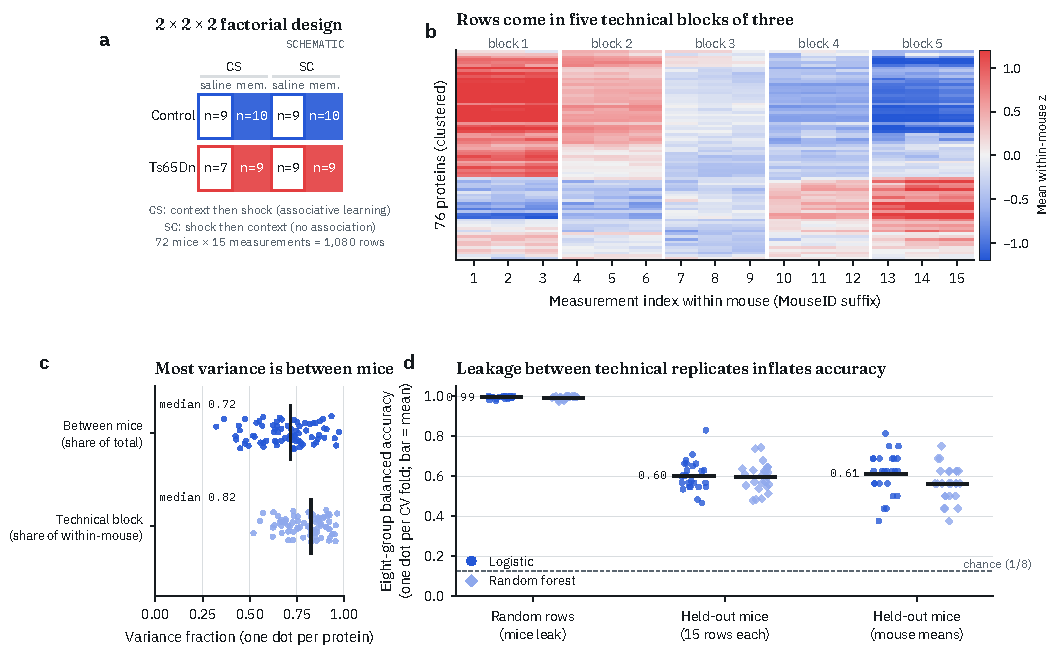
\includegraphics[width=\linewidth]{../results/mechanisms/figures/fig1_design_qc.pdf}
\caption{\textbf{Experimental design and measurement structure.}
\textbf{a}, Schematic of the factorial design; numbers are mice per cell, counted from the data.
\textbf{b}, Mean within-mouse $z$-score of each protein at each measurement index (columns),
averaged over mice; proteins are clustered. Indices 1--3, 4--6, \ldots, 13--15 form five
technical blocks.
\textbf{c}, Variance decomposition of log$_2$ levels for \NUnique{} proteins: between-mouse
share of total variance, and the share of within-mouse variance explained by technical block.
\textbf{d}, Eight-group balanced accuracy for each cross-validation fold (5 repeats $\times$
5 folds) under three validation designs; bars are means. Random row splits place measurements
of the same mouse in training and test sets.}
\label{fig:design}
\end{figure}

\subsection{Q1. Triplicated proteins rise, but far below gene dosage}
\textit{Question: do three gene copies give 1.5 times as much protein? Answer: the increase is
about a quarter of that, and it tracks copy number.}

\begin{figure}[t]
\centering
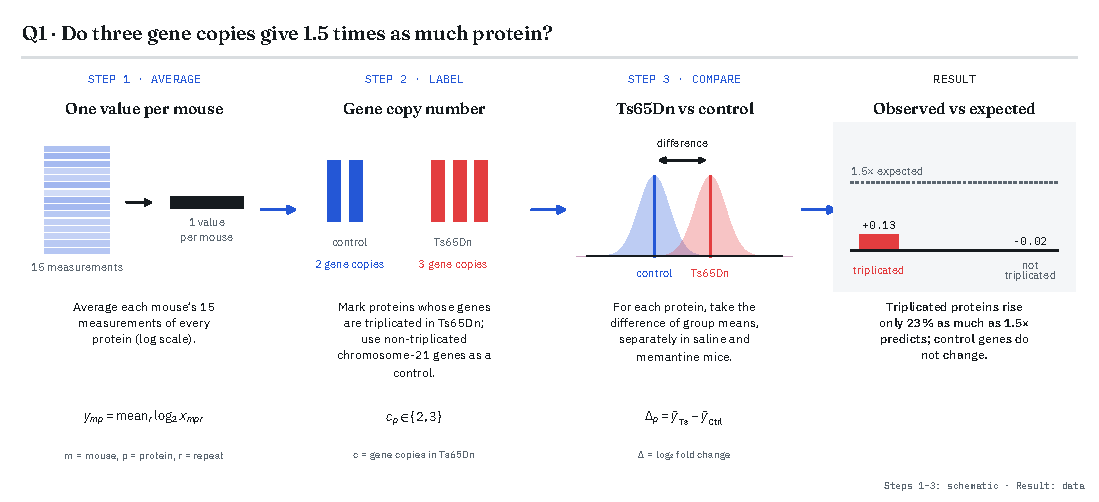
\includegraphics[width=\linewidth]{../results/mechanisms/figures/workflows/wf_q1_dosage.pdf}
\caption{\textbf{Workflow for Q1 (gene dosage).} Each step shows its
defining equation; the last step states the result. Schematic; numbers are generated from the
results.}
\label{fig:wfq1}
\end{figure}

Under strict gene dosage, proteins encoded in the triplicated segment would be 1.5-fold
(\DosageExpected{} log$_2$ units) higher in Ts65Dn mice. Averaged over the six measured
triplicated proteins and all \NMice{} mice, the increase was \DosageTri{} log$_2$ units (95\%
bootstrap CI \DosageTriCI{}; a \DosageFold-fold change), \DosageFrac\% of the expectation
(\figref{fig:dosage}c). Two HSA21 orthologs that are \emph{not} triplicated in Ts65Dn
(\tech{RRP1}, \tech{ADARB1}) acted as a negative control and were unchanged (\DosageDis{};
\DosageDisCI), as were the \NBackground{} other panel proteins (\DosageBg{}; \DosageBgCI).

The effect was uneven across genes (\figref{fig:dosage}a). APP (\APPfc), ITSN1 (\ITSNfc) and
DYRK1A (\DYRKfc{} log$_2$FC in saline mice) were among the most increased proteins in the panel,
whereas SOD1 (\SODfc), DSCR1/RCAN1 (\DSCRfc) and TIAM1 (\TIAMfc) were not increased. Only
\DosageQSig{} triplicated protein passed FDR 5\% individually, so the gene-level pattern is
descriptive. Fold changes estimated in saline mice and, independently, in memantine-treated
mice agreed across proteins (Pearson $r = \DosageRep$; \figref{fig:dosage}b), which shows that
the estimates are reproducible across disjoint animals.

The attenuation has several non-exclusive explanations: compression of the dynamic range in
antibody-based arrays, measurement in a nuclear fraction that does not reflect total cellular
protein, and post-transcriptional dosage compensation. These data cannot separate them.

\begin{figure}[t]
\centering
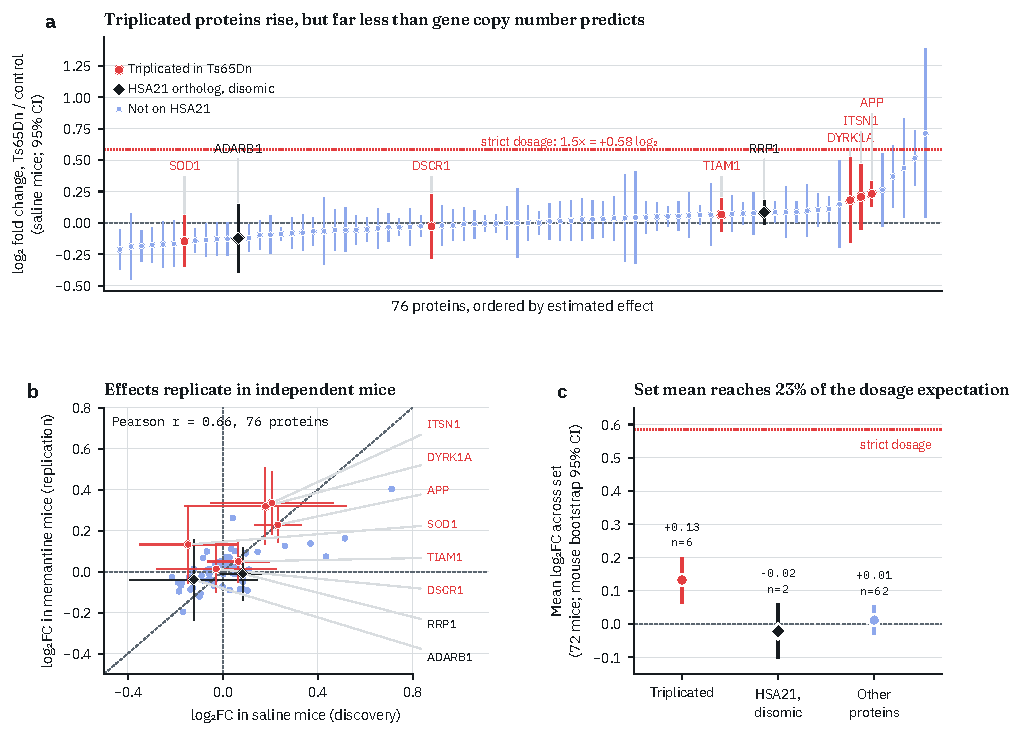
\includegraphics[width=\linewidth]{../results/mechanisms/figures/fig2_gene_dosage.pdf}
\caption{\textbf{Gene dosage.}
\textbf{a}, Ts65Dn/control log$_2$ fold change of each protein in saline-treated mice (Welch
contrast averaged over conditioning; 95\% CI). Dotted line: 1.5-fold strict-dosage expectation.
\textbf{b}, Fold changes estimated from disjoint sets of mice: saline (discovery) versus
memantine (replication). Dashed line: identity.
\textbf{c}, Mean fold change of each protein set over all \NMice{} mice, with 95\% intervals from
\NBoot{} stratified mouse bootstrap resamples.}
\label{fig:dosage}
\end{figure}

\subsection{Q2. Trisomy and treatment alter a conditioning-associated signature}
\textit{Question: does trisomy change the protein response to learning? Answer: the response
projects less strongly in untreated trisomic mice; the treated estimate is near control.}

\begin{figure}[t]
\centering
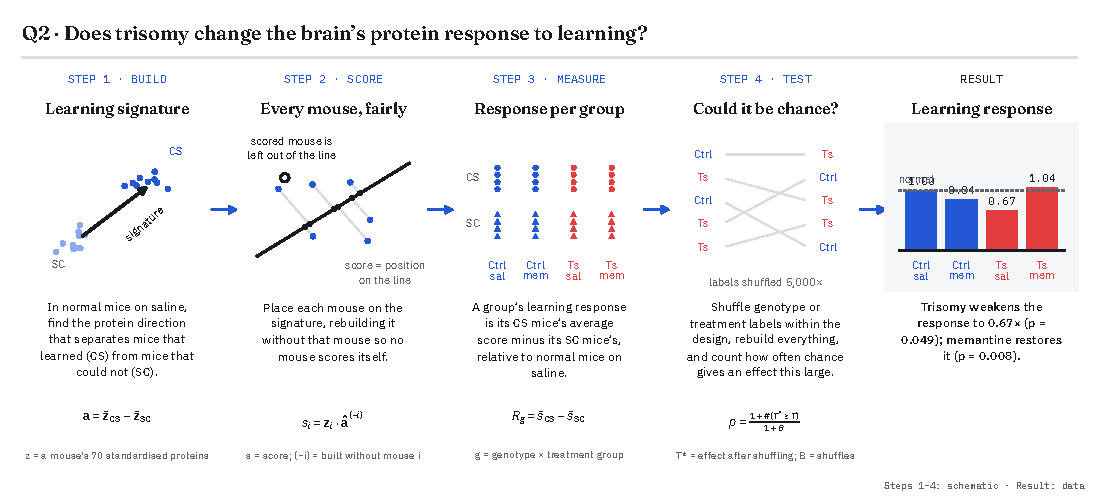
\includegraphics[width=\linewidth]{../results/mechanisms/figures/workflows/wf_q2_learning.pdf}
\caption{\textbf{Workflow for Q2 (the learning response).} Each step shows its
defining equation; the last step states the result. Schematic; numbers are generated from the
results.}
\label{fig:wfq2}
\end{figure}

Conditioning order is the strongest experimental signal in the data: \NCond{} of \NUnique{}
proteins differ between CS and SC at FDR 5\%, against \NGeno{} for genotype and \NTreat{} for
treatment. To ask whether trisomy changes the response to conditioning, we defined a reference
axis as the CS$-$SC difference of mean profiles in saline-treated control mice and projected
every mouse onto it, using a leave-one-out axis for the mice that define it (Methods). The axis
is dominated by \LearnTopProteins{} (\figref{fig:learning}d).

All four arms separated CS from SC along this axis (\figref{fig:learning}a), but by different
amounts. Relative to control-saline mice, the response was \LearnRelTsSal{} in saline-treated
Ts65Dn mice (95\% CI \LearnRelTsSalCI; permutation $p = \LearnAttP$ for the difference),
\LearnRelTsMem{} in memantine-treated Ts65Dn mice (\LearnRelTsMemCI; $p = \LearnResP$ for the
specified contrast) and \LearnRelCtrlMem{} in memantine-treated controls (\LearnRelCtrlMemCI;
\figref{fig:learning}b). The direction of the response was preserved: noise-corrected cosine
similarities with the control-saline response were \CosTsSal{} (Ts65Dn saline; \CosTsSalCI),
\CosTsMem{} (Ts65Dn memantine) and \CosCtrlMem{} (control memantine; \figref{fig:learning}c).
At the level of single proteins the same pattern appears as a drop in the number of CS--SC
differences, from \NLearnCS{} in control-saline mice to \NLearnTS{} in Ts65Dn-saline mice and
\NLearnTM{} in Ts65Dn-memantine mice (FDR 5\%), although per-protein counts conflate effect size
with power.

Thus saline-treated Ts65Dn mice show a weaker projection on this control-defined axis,
while the treated estimate is near the control reference. This does not establish the same
protein response or equivalence between groups. The pattern is consistent with the behavioural phenotype
reported for these animals: Ts65Dn mice failed context fear conditioning and memantine rescued
it \cite{costa2008, ahmed2015}. The workbook does not contain individual behavioural scores, so
the link to learning is at the level of groups, not individual mice.

\begin{figure}[t]
\centering
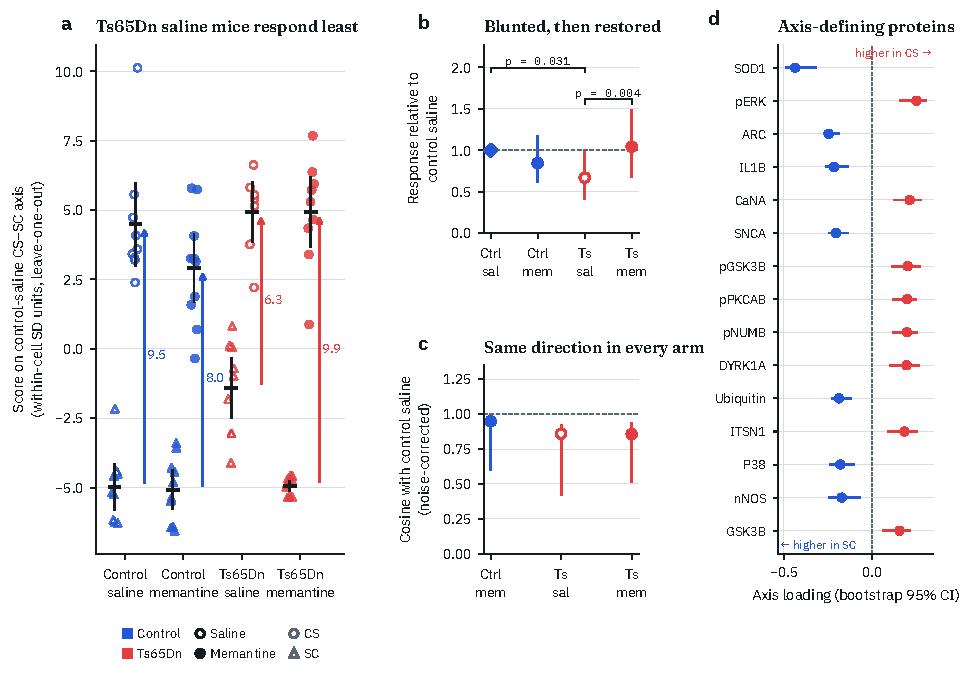
\includegraphics[width=\linewidth]{../results/mechanisms/figures/fig3_learning_signature.pdf}
\caption{\textbf{A multivariate conditioning signature.}
\textbf{a}, Each mouse projected on the reference CS$-$SC axis defined in control-saline mice
(within-cell SD units; mice defining the axis are scored on a leave-one-out axis). Bars: cell
means and 95\% CIs; arrows and numbers: CS$-$SC response of each arm.
\textbf{b}, Response relative to control saline, with 95\% stratified bootstrap CIs and
one-sided permutation $p$-values (genotype permuted among saline mice; treatment permuted among
Ts65Dn mice; \NPerm{} permutations each, recomputing the axis).
\textbf{c}, Cosine between each arm's CS$-$SC vector and the control-saline vector, corrected
for sampling noise.
\textbf{d}, The 15 largest axis loadings with bootstrap 95\% CIs.}
\label{fig:learning}
\end{figure}

\subsection{Q3. Memantine moves Ts65Dn mice toward control, but not selectively}
\textit{Question: does memantine reverse the trisomic profile? Answer: partly, but it moves
control mice the same way, so it is not a trisomy-specific repair.}

\begin{figure}[t]
\centering
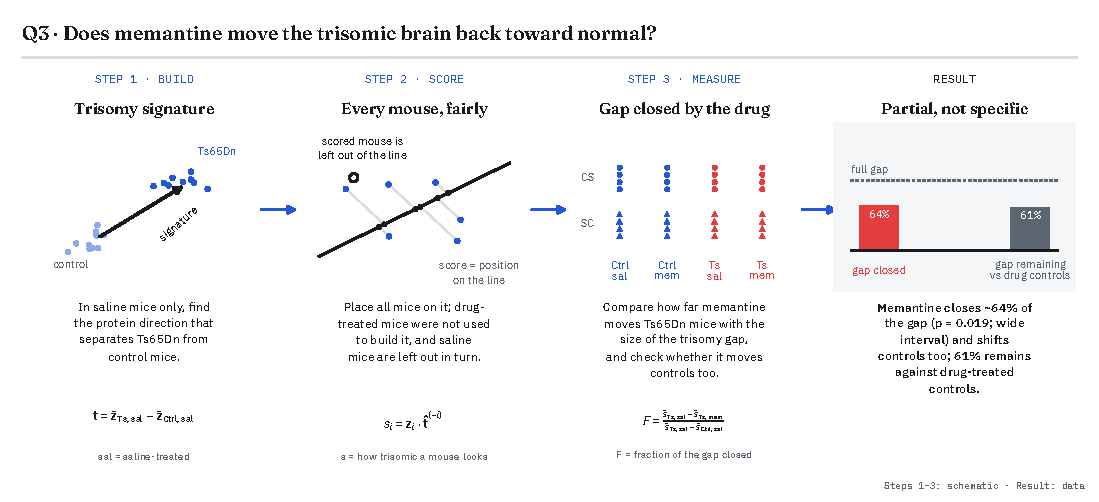
\includegraphics[width=\linewidth]{../results/mechanisms/figures/workflows/wf_q3_rescue.pdf}
\caption{\textbf{Workflow for Q3 (memantine rescue).} Each step shows its
defining equation; the last step states the result. Schematic; numbers are generated from the
results.}
\label{fig:wfq3}
\end{figure}

The trisomy axis was defined as the Ts65Dn$-$control difference among saline mice, averaged over
conditioning. Saline Ts65Dn mice lay well above saline controls on this axis, and memantine moved
Ts65Dn mice back toward them (\figref{fig:rescue}a), closing \RescueFrac\% of the gap (95\% CI
\RescueFracCI; permutation $p = \RescueP$ against no memantine effect in Ts65Dn mice). The
apparent rescue was larger in SC (\RescueSC; \RescueSCCI) than in CS mice (\RescueCS; CI
\RescueCSCI), where the saline trisomy gap was too small to estimate a ratio reliably.

Two observations argue against a genotype-specific normalisation. First, memantine also shifted
control mice along the same axis (shift \CtrlShift{} of the saline gap; \CtrlShiftCI), so
relative to memantine-treated controls \Persist\% of the trisomy gap remained (\PersistCI;
\figref{fig:rescue}b). Second, the drug effect in Ts65Dn mice was large in absolute terms
(noise-corrected magnitude \MagDrugTs{} SD, against \MagTri{} SD for trisomy and \MagDrugCtrl{}
SD for memantine in controls; \figref{fig:rescue}c), and only about \AxisShare\% of it lay along
the trisomy axis (\AxisShareCI). Most of what memantine does to the Ts65Dn proteome is therefore
something other than reversing trisomy.

Protein-level analysis agrees. Comparing each protein's trisomy effect in saline mice with the
same effect measured in independent memantine-treated mice, the error-corrected slope was
\SlopeCorr{} (naive slope \SlopeNaive; reliability \Reliability), close to the value of 1 that
means no rescue (\figref{fig:rescue}d). Only \NAffected{} proteins had a trisomy effect at FDR 5\%
in saline mice, which is too few for a gene-by-gene rescue map.

\begin{figure}[t]
\centering
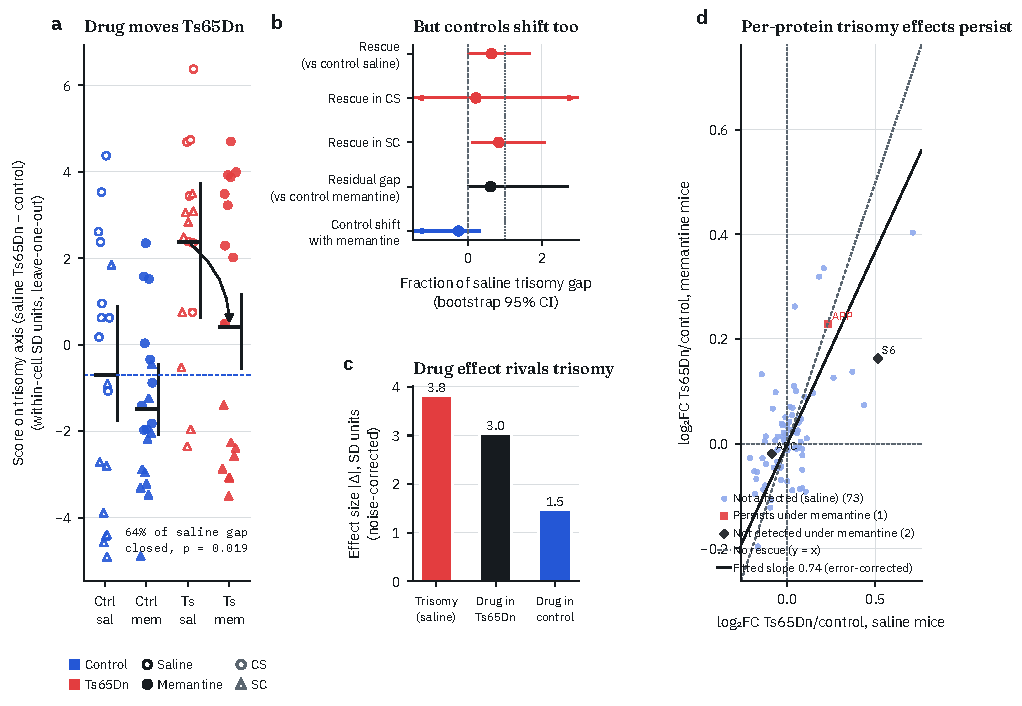
\includegraphics[width=\linewidth]{../results/mechanisms/figures/fig4_rescue.pdf}
\caption{\textbf{Memantine and the trisomy axis.}
\textbf{a}, Each mouse projected on the trisomy axis (saline Ts65Dn minus saline control,
averaged over conditioning; saline mice scored leave-one-out). Bars: arm means with bootstrap
95\% CIs; dashed line: control-saline mean. The $p$-value tests the Ts65Dn saline$-$memantine
shift against permutation of treatment among Ts65Dn mice.
\textbf{b}, Ratios expressed as fractions of the saline trisomy gap (bootstrap 95\% CIs; arrows
mark intervals beyond the axis).
\textbf{c}, Euclidean magnitude of each effect across \NPanel{} proteins, corrected for noise.
\textbf{d}, Per-protein trisomy effects estimated in saline versus memantine mice (disjoint
animals). Points on the identity line indicate no rescue; the solid line is the slope corrected
for measurement error in the $x$ estimates.}
\label{fig:rescue}
\end{figure}

\subsection{Signalling activity follows conditioning more than genotype}
\textit{Question: which signalling pathways respond? Answer: mainly those linked to
conditioning; genotype effects on pathway activity are small.}

For 17 proteins the panel measures both a phospho-form and the total protein, so their log-ratio
indexes how much of the protein is phosphorylated. Averaged into seven pathway scores, the
largest effects were again those of conditioning: CS mice had lower JNK, CaMKII--CREB, NMDA
receptor and AKT--mTOR phosphorylation indices and a higher PKC index than SC mice
(\figref{fig:pathways}; Table~\ref{tab:pathways}). Memantine raised the MAPK/ERK index and lowered
the PKC index. JNK showed a genotype $\times$ treatment interaction, and the NMDA receptor score a
genotype $\times$ conditioning interaction. Member ratios within a pathway were nearly
uncorrelated across mice (Table~\ref{tab:pathways}, footnote), so pathway scores are averages of
largely independent readouts, and the ratio-level view (\figref{fig:pathways}b) is the more
faithful description.

\begin{figure}[t]
\centering
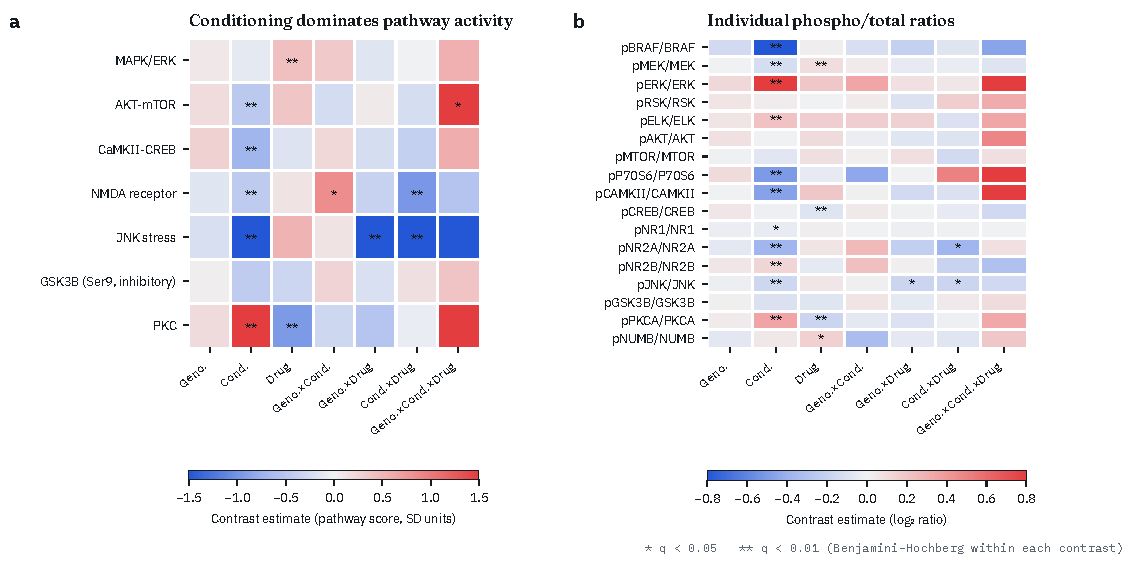
\includegraphics[width=\linewidth]{../results/mechanisms/figures/fig5_pathways.pdf}
\caption{\textbf{Phosphorylation-based activity indices.}
\textbf{a}, Factorial contrasts for seven pathway scores (mean of standardised phospho/total
log-ratios; within-cell SD units).
\textbf{b}, The same contrasts for each of the 17 log$_2$ phospho/total ratios. Main effects are
differences of level means; interactions are average differences of differences. Asterisks:
Benjamini--Hochberg $q$ within each contrast.}
\label{fig:pathways}
\end{figure}

\begin{table}[t]
\centering
\caption{\textbf{Pathway contrasts significant at FDR 5\%.}}
\label{tab:pathways}
\small
\begin{tabular}{llrrr}
\toprule
Pathway & Contrast & Estimate (SD) & 95\% CI & $q$ \\
\midrule
PKC & Conditioning & +1.87 & [+1.38, +2.35] & 1.2e-08 \\
JNK stress & Conditioning & -1.63 & [-2.12, -1.13] & 2.1e-07 \\
CaMKII-CREB & Conditioning & -0.70 & [-1.04, -0.35] & 0.00036 \\
NMDA receptor & Conditioning & -0.45 & [-0.72, -0.18] & 0.0034 \\
AKT-mTOR & Conditioning & -0.47 & [-0.80, -0.14] & 0.01 \\
NMDA receptor & Conditioning$\times$Treatment & -0.97 & [-1.52, -0.42] & 0.0033 \\
JNK stress & Conditioning$\times$Treatment & -1.74 & [-2.73, -0.76] & 0.0033 \\
NMDA receptor & Genotype$\times$Conditioning & +0.85 & [+0.30, +1.40] & 0.023 \\
AKT-mTOR & Genotype$\times$Conditioning$\times$Treatment & +1.94 & [+0.61, +3.27] & 0.041 \\
JNK stress & Genotype$\times$Treatment & -1.78 & [-2.77, -0.80] & 0.0053 \\
MAPK/ERK & Treatment & +0.42 & [+0.22, +0.62] & 0.00082 \\
PKC & Treatment & -0.94 & [-1.43, -0.46] & 0.0012 \\
\bottomrule
\end{tabular}
\par\smallskip{\footnotesize Mean within-cell correlation of member ratios: MAPK/ERK -0.04; AKT-mTOR +0.11; CaMKII-CREB +0.06; NMDA receptor -0.03.}

\end{table}

\subsection{Q4. No evidence that trisomy rewires protein networks}
\textit{Question: do proteins co-vary differently in trisomic mice? Answer: we found no
evidence, although only large changes were detectable.}

\begin{figure}[t]
\centering
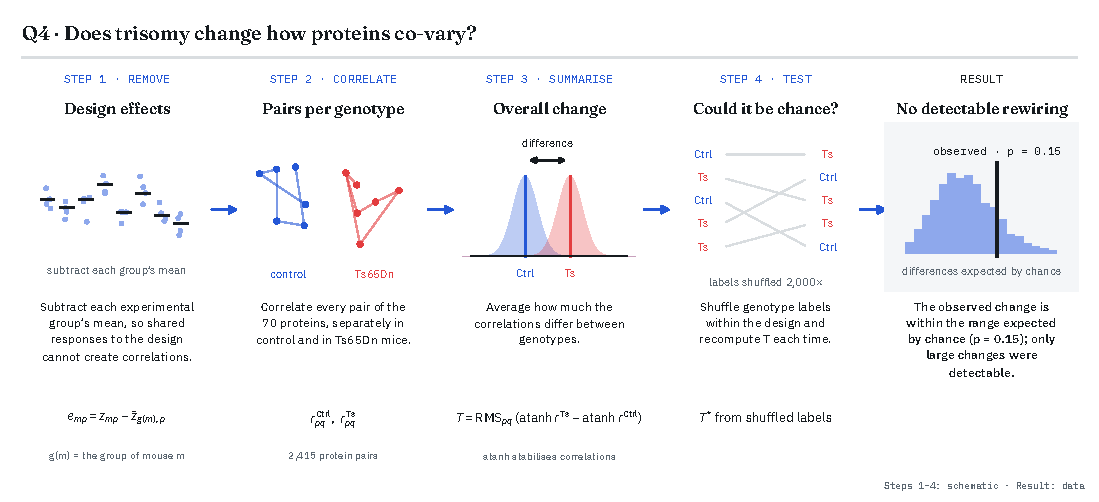
\includegraphics[width=\linewidth]{../results/mechanisms/figures/workflows/wf_q4_network.pdf}
\caption{\textbf{Workflow for Q4 (network rewiring).} Each step shows its
defining equation; the last step states the result. Schematic; numbers are generated from the
results.}
\label{fig:wfq4}
\end{figure}

Trisomy could change how proteins co-vary without changing their means. After removing the eight
cell means, residual correlation matrices were similar in the two genotypes
(\figref{fig:network}a). The root-mean-square difference of Fisher-transformed correlations
(\NetStat) did not exceed its permutation null (mean \NetNull; $p = \NetP$;
\figref{fig:network}c), and none of the \NetPairs{} protein pairs differed at FDR 5\%
(\figref{fig:network}b). With 30--34 residual degrees of freedom per genotype only large
rewiring would be detectable, so this is an absence of evidence rather than evidence of absence.

\begin{figure}[t]
\centering
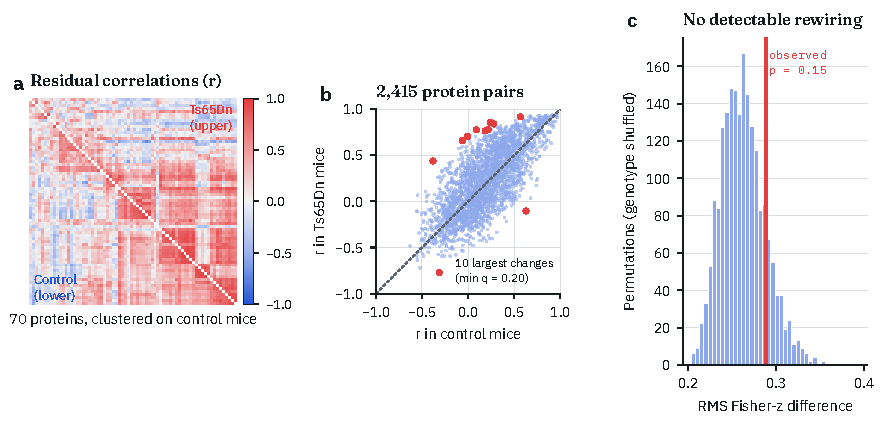
\includegraphics[width=\linewidth]{../results/mechanisms/figures/fig6_network.pdf}
\caption{\textbf{Network rewiring.}
\textbf{a}, Correlation of cell-mean-centred protein levels in control (lower triangle) and
Ts65Dn mice (upper triangle), ordered by clustering of the control matrix.
\textbf{b}, Correlation of every protein pair in each genotype; highlighted: the ten largest
Fisher-$z$ differences.
\textbf{c}, Global rewiring statistic against \NNetPerm{} permutations of genotype within
treatment $\times$ conditioning strata (residuals recomputed for each permutation).}
\label{fig:network}
\end{figure}

\subsection{What a follow-up experiment needs}
\textit{Question: how large must the next study be? Answer: about ten mice per group for the
learning effect; many more for single-protein interactions.}

Using the observed within-cell variability of the conditioning score (SD \LearnSD), a study with
nine mice per cell has \PowAttNine\% power to detect the observed attenuation of the conditioning
response, and ten mice per cell reach 80\% (\figref{fig:power}). Interactions at the level of a
single protein are much harder: a three-way interaction of one within-cell SD has
\PowThreeOneNine\% power at nine mice per cell and needs \NThreeOne{} per cell for 80\%; a 2-SD
interaction needs \NThreeTwo. Projected, multivariate endpoints are therefore the efficient
primary outcome for studies of this size.

\begin{figure}[t]
\centering
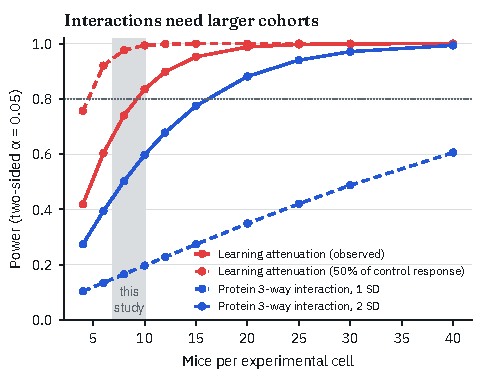
\includegraphics[width=0.62\linewidth]{../results/mechanisms/figures/fig7_power.pdf}
\caption{\textbf{Power of a follow-up study.} Two-sided power ($\alpha = 0.05$) of planned
contrasts as a function of mice per cell, from the non-central $t$ distribution. Learning
attenuation uses the observed effect and within-cell SD of the conditioning score; protein
three-way interactions are in within-cell SD units. Shaded band: cell sizes in this study.}
\label{fig:power}
\end{figure}

\subsection{Prediction from held-out mice}
Table~\ref{tab:validation} summarises the leakage audit: with whole mice held out, logistic
regression and random forests reach similar accuracy, far below the near-perfect scores of
random row splits. A separate study in this repository (\texttt{foundation\_models/}) compares
pretrained tabular foundation models with tuned conventional models on these data.

\begin{table}[t]
\centering
\caption{\textbf{Eight-group balanced accuracy under three validation designs.} Mean and SD
over five repeats of five-fold cross-validation.}
\label{tab:validation}
\small
\begin{tabular}{llrr}
\toprule
Validation & Model & Balanced accuracy & SD \\
\midrule
Random rows (leaky) & Logistic & 0.994 & 0.006 \\
Held-out mice, 15 rows & Logistic & 0.602 & 0.076 \\
Held-out mice, 15 rows & Random forest & 0.596 & 0.070 \\
Held-out mice, means & Logistic & 0.613 & 0.105 \\
\midrule
Held-out mice, means & Elastic net & 0.630 & 0.024 \\
Held-out mice, means & RBF SVM & 0.540 & 0.030 \\
Held-out mice, means & Gradient boosting & 0.557 & 0.042 \\
Held-out mice, means & TabPFN v2$^\dagger$ & 0.730 & 0.032 \\
Held-out mice, means & Kumo Tabular Small$^\dagger$ & 0.828 & 0.022 \\
Chance & -- & 0.125 & -- \\
\bottomrule
\end{tabular}

\end{table}

% ================================================================ 3
\section{Discussion}

We set out to answer four questions that the usual benchmark use of this dataset leaves open.
Analysed as an experiment, with the mouse as the unit, the data give the following answers.
\begin{enumerate}[label=\textbf{Q\arabic*.}, leftmargin=2.6em]
\item \textbf{Gene dosage.} Six selected triplicated-gene proteins show a mean log$_2$
  difference smaller than the simple dosage expectation; this does not describe all genes.
\item \textbf{Conditioning.} Untreated trisomic mice project less strongly on a control-defined
  conditioning axis. The treated estimate is near control, without proving restoration.
\item \textbf{Rescue.} The signature shift toward controls has wide uncertainty and does not
  establish a genotype-specific drug effect.
\item \textbf{Networks.} No covariance difference was detected; modest changes remain possible.
\end{enumerate}

The answer to Q2 is the most biologically specific. It links a molecular measure to the
known behavioural phenotype without using behavioural data, and it is robust to the choice of
estimator: projections use leave-one-out axes and the reference arm is not compared with itself.
However, label-dependent pooled standardization uses all mice and is held fixed in resampling,
so the scores are not fully out-of-sample and the permutation inference is conditional on
observed scaling. The effect is moderate
(attenuation $p = \LearnAttP$; the upper confidence limit of the relative response is near 1),
and should be treated as a well-motivated hypothesis for replication rather than an
established fact.

\paragraph{Methodological lessons} Three general points emerge. (1) Technical replicates must be
aggregated or modelled; ignoring them changes accuracy from \GroupedBA{} to \RowBA. (2) Selecting
proteins on an effect and then estimating a second effect from the same animals manufactures
apparent rescue through regression to the mean; estimating the two effects in disjoint animals,
or using leave-one-out projections, avoids it. (3) Raw cosines and Euclidean norms of noisy
difference vectors are biased toward 0 and upward respectively; the noise corrections used here
are simple and unbiased.

\paragraph{Limitations} All mice were male and came from one laboratory, protocol and assay; no
external cohort exists. CS versus SC differs in timing as well as in associative content, so the
conditioning axis captures the protocol and not learning alone. The dilution and replicate
structure is inferred, not documented. Pathway scores rely on antibody-specific ratios that are
not stoichiometries. Gene annotations for the triplicated segment follow published breakpoint
mapping \cite{duchon2011, reinholdt2011}, and a different gene set would change the dosage
estimates.

% ================================================================ 4
\section{Methods}

\paragraph{Data} We used the original UCI workbook (\tech{Data\_Cortex\_Nuclear.xls}; SHA-256
recorded in the repository) \cite{uci2015}. The animal identifier is the \tech{MouseID} prefix
before the final underscore; a data contract test verifies \NMice{} animals with exactly 15 rows
each and constant labels within animals. One non-positive value was treated as missing.

\paragraph{Mouse-level values} For each mouse and protein we averaged log$_2$ intensities over
available rows (the log of the geometric mean). Group differences are therefore log$_2$ fold
changes. For multivariate analyses each protein was centred at the grand mean and scaled by the
pooled within-cell SD, so one unit is one SD of biological variation between mice of the same
cell; the \NImputed{} missing mouse means in the \NPanel-protein panel were set to 0, a choice
that does not use labels.

\paragraph{Planned contrasts} Every group comparison is a contrast $L = \sum_c w_c \bar y_c$ over
the eight cell means, with Welch standard error $\mathrm{SE}(L) = \big(\sum_c w_c^2
s_c^2/n_c\big)^{1/2}$ and Welch--Satterthwaite degrees of freedom \cite{welch1947}. Main effects
use weights $\pm 1/4$ (difference of level means), two-way interactions $\pm 1/2$ (average
difference of differences) and the three-way interaction $\pm 1$. False discovery rates use the
Benjamini--Hochberg procedure within each contrast \cite{bh1995}.

\paragraph{Axis projections} An axis is a contrast of cell-mean profiles, $\mathbf a = \sum_c
w_c \bar{\mathbf z}_c$; a mouse is scored by $s_i = \mathbf z_i^\top \mathbf a / \lVert\mathbf
a\rVert$. A mouse in a cell with $w_c \neq 0$ is scored on the axis re-estimated without it,
$\mathbf a^{(-i)} = \mathbf a + w_c\,(\bar{\mathbf z}_c - \mathbf z_i)/(n_c - 1)$, which removes
self-projection bias at the cost of one pass. Within bootstrap resamples all copies of a mouse
are left out together. The conditioning axis uses $w = (+1, -1)$ on control-saline CS and SC
cells; the trisomy axis uses $\pm 1/2$ on the four saline cells. The rescue fraction is
$(\bar s_{\mathrm{Ts,sal}} - \bar s_{\mathrm{Ts,mem}}) / (\bar s_{\mathrm{Ts,sal}} - \bar
s_{\mathrm{Ctrl,sal}})$, where arm means average the CS and SC cells equally.

\paragraph{Noise-corrected magnitudes and cosines} For a contrast vector $\hat{\mathbf d}$ of
cell means, $\mathbb E\lVert \hat{\mathbf d}\rVert^2 = \lVert\mathbf d\rVert^2 + \sum_c w_c^2
\operatorname{tr}(\boldsymbol\Sigma_c)/n_c$; subtracting the unbiased estimate of the second
term gives an unbiased squared magnitude. For contrasts on disjoint cells the inner product is
unbiased, and dividing it by the corrected norms gives a cosine free of the attenuation that
noise induces (the multivariate analogue of Spearman's correction \cite{spearman1904}).

\paragraph{Per-protein persistence} The trisomy effect of each protein was estimated separately
in saline and in memantine mice (disjoint animals). The slope of memantine on saline estimates
across proteins was divided by the reliability of the saline estimates, $\lambda = 1 -
\overline{\mathrm{SE}^2}/\operatorname{Var}(\hat\beta_{\mathrm{sal}})$, to correct regression
dilution \cite{fuller1987}. We deliberately did not classify proteins as ``rescued'' by testing
the Ts65Dn memantine$-$saline difference among proteins selected on the Ts65Dn$-$control
difference in saline mice: both estimates share the Ts65Dn-saline cell, which creates spurious
rescue through regression to the mean.

\paragraph{Resampling} Confidence intervals are percentile intervals from \NBoot{} bootstrap
resamples of mice within cells \cite{efron1993}. Permutation tests shuffle one factor among mice
within strata of the other two factors and recompute the entire analysis, axis included
(\NPerm{} permutations; $p = (1 + \#\{T^* \ge T\})/(1 + B)$).

\paragraph{Pathways} Log-ratios $\log_2(\text{phospho}) - \log_2(\text{total})$ were formed for
17 pairs. Pathway scores average standardised member ratios. \tech{pS6} was excluded because it
duplicates \tech{ARC}.

\paragraph{Network rewiring} Correlations were computed within genotype on residuals after
removing the eight cell means. The global statistic is the root-mean-square difference in
Fisher-$z$ over all pairs, compared with \NNetPerm{} genotype permutations within treatment
$\times$ conditioning strata. Pairwise tests use Fisher's $z$ with $n-4$ effective observations
per genotype.

\paragraph{Power} Power for a contrast with common SD $\sigma$ and $n$ mice per cell uses the
non-central $t$ distribution with non-centrality $L/(\sigma\sqrt{\sum w_c^2/n})$ and pooled
residual degrees of freedom; it agrees with Monte Carlo simulation in the test suite.

\paragraph{Prediction} Prediction results use five repeats of five-fold cross-validation
stratified on the eight groups, with all preprocessing fitted inside training folds.

\paragraph{Software and reproducibility} Analyses used Python \PyVersion{} with scikit-learn
\SklearnVersion, NumPy, pandas, SciPy and statsmodels; the random seed is \Seed. Tests check data
contracts, leakage-safe splitting, the closed-form leave-one-out projection against brute-force
refitting, unbiasedness of the noise corrections, recovery of a simulated 50\% rescue, Welch
contrasts against SciPy, and analytic power against simulation. \texttt{make reproduce}
regenerates all results, figures and this article.

\section*{Data and code availability}
The UCI dataset is distributed under CC BY 4.0 \cite{uci2015}. All code, configuration, tests and
results are in the accompanying repository.

% ---------------------------------------------------------------- references
\begingroup
\small
\begin{thebibliography}{99}
\setlength{\itemsep}{0.15em}
\bibitem{ahmed2015} Ahmed MM, Dhanasekaran AR, Block A, Tong S, Costa ACS, Stasko M, Gardiner KJ.
Protein dynamics associated with failed and rescued learning in the Ts65Dn mouse model of Down
syndrome. \emph{PLoS ONE} 10, e0119491 (2015).
\bibitem{higuera2015} Higuera C, Gardiner KJ, Cios KJ. Self-organizing feature maps identify
proteins critical to learning in a mouse model of Down syndrome. \emph{PLoS ONE} 10, e0129126
(2015).
\bibitem{uci2015} Higuera C, Gardiner K, Cios K. Mice Protein Expression [dataset]. UCI Machine
Learning Repository (2015). doi:10.24432/C50S3Z. \url{https://archive.ics.uci.edu/dataset/342/mice+protein+expression}.
\bibitem{reeves1995} Reeves RH, Irving NG, Moran TH, et al. A mouse model for Down syndrome
exhibits learning and behaviour deficits. \emph{Nat. Genet.} 11, 177--184 (1995).
\bibitem{duchon2011} Duchon A, Raveau M, Chevalier C, et al. Identification of the translocation
breakpoints in the Ts65Dn and Ts1Cje mouse lines: relevance for modeling Down syndrome.
\emph{Mamm. Genome} 22, 674--684 (2011).
\bibitem{reinholdt2011} Reinholdt LG, Ding Y, Gilbert GJ, et al. Molecular characterization of the
translocation breakpoints in the Down syndrome mouse model Ts65Dn. \emph{Mamm. Genome} 22,
685--691 (2011).
\bibitem{costa2008} Costa ACS, Scott-McKean JJ, Stasko MR. Acute injections of the NMDA receptor
antagonist memantine rescue performance deficits of the Ts65Dn mouse model of Down syndrome on a
fear conditioning test. \emph{Neuropsychopharmacology} 33, 1624--1632 (2008).
\bibitem{lazic2010} Lazic SE. The problem of pseudoreplication in neuroscientific studies: is it
affecting your analysis? \emph{BMC Neurosci.} 11, 5 (2010).
\bibitem{kaufman2012} Kaufman S, Rosset S, Perlich C, Stitelman O. Leakage in data mining:
formulation, detection, and avoidance. \emph{ACM Trans. Knowl. Discov. Data} 6, 15 (2012).
\bibitem{tibes2006} Tibes R, Qiu Y, Lu Y, et al. Reverse phase protein array: validation of a novel
proteomic technology and utility for analysis of primary leukemia specimens and hematopoietic
stem cells. \emph{Mol. Cancer Ther.} 5, 2512--2521 (2006).
\bibitem{welch1947} Welch BL. The generalization of ``Student's'' problem when several different
population variances are involved. \emph{Biometrika} 34, 28--35 (1947).
\bibitem{bh1995} Benjamini Y, Hochberg Y. Controlling the false discovery rate: a practical and
powerful approach to multiple testing. \emph{J. R. Stat. Soc. B} 57, 289--300 (1995).
\bibitem{spearman1904} Spearman C. The proof and measurement of association between two things.
\emph{Am. J. Psychol.} 15, 72--101 (1904).
\bibitem{fuller1987} Fuller WA. \emph{Measurement Error Models}. Wiley (1987).
\bibitem{efron1993} Efron B, Tibshirani RJ. \emph{An Introduction to the Bootstrap}. Chapman \&
Hall (1993).
\end{thebibliography}
\endgroup

% ---------------------------------------------------------------- supplement
\clearpage
\renewcommand{\thefigure}{S\arabic{figure}}
\setcounter{figure}{0}
\section*{Supplementary information}

\begin{figure}[H]
\centering
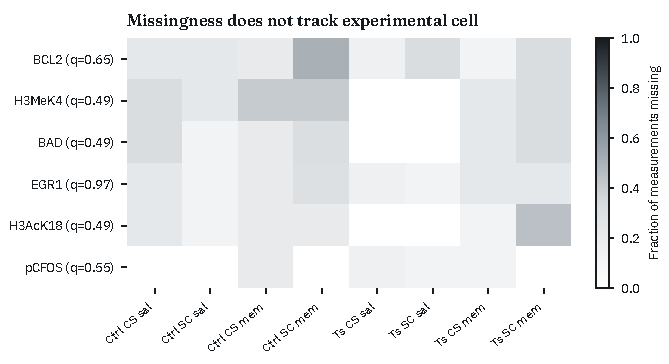
\includegraphics[width=0.7\linewidth]{../results/mechanisms/figures/figS1_missingness.pdf}
\caption{\textbf{Missingness by experimental cell} for the six proteins with substantial missing
data. Shade: fraction of a cell's measurements missing. $q$: Benjamini--Hochberg-adjusted
Kruskal--Wallis test of the per-mouse missing fraction across cells.}
\label{fig:missing}
\end{figure}



\end{document}
